\documentclass{article}
\usepackage[english,russian]{babel}
\usepackage{textcomp}
\usepackage{geometry}
  \geometry{left=2cm}
  \geometry{right=1.5cm}
  \geometry{top=1.5cm}
  \geometry{bottom=2cm}
\usepackage{tikz}
\usepackage{multicol}
\usepackage{listings}
\pagenumbering{gobble}

\lstdefinestyle{csMiptCppStyle}{
  language=C++,
  basicstyle=\linespread{1.1}\ttfamily,
  columns=fixed,
  fontadjust=true,
  basewidth=0.5em,
  keywordstyle=\color{blue}\bfseries,
  commentstyle=\color{gray},
  texcl=true,
  stringstyle=\ttfamily\color{orange!50!black},
  showstringspaces=false,
  numbersep=5pt,
  numberstyle=\tiny\color{black},
  numberfirstline=true,
  stepnumber=1,      
  numbersep=10pt,
  backgroundcolor=\color{white},
  showstringspaces=false,
  captionpos=b,
  breaklines=true
  breakatwhitespace=true,
  xleftmargin=.2in,
  extendedchars=\true,
  keepspaces = true,
  tabsize=4,
  upquote=true,
}


\lstdefinestyle{csMiptCppLinesStyle}{
  style=csMiptCppStyle,
  frame=lines,
}

\lstdefinestyle{csMiptCppBorderStyle}{
  style=csMiptCppStyle,
  framexleftmargin=5mm, 
  frame=shadowbox, 
  rulesepcolor=\color{gray}
}

\lstset{style=csMiptCppStyle}
\lstset{literate={~}{{\raisebox{0.5ex}{\texttildelow}}}{1}}


\renewcommand{\thesection}{\arabic{section}}
\makeatletter
\def\@seccntformat#1{\@ifundefined{#1@cntformat}%
   {\csname the#1\endcsname\quad}%    default
   {\csname #1@cntformat\endcsname}}% enable individual control
\newcommand\section@cntformat{Часть \thesection:\space}
\makeatother

\begin{document}
\title{Семинар \#2: Наследование. \vspace{-5ex}}\date{}\maketitle
\section{Основы наследования}
Наследование (англ. \textit{inheritance}) -- это механизм, позволяющий создавать новый класс на основе существующего класса (или классов), заимствуя его свойства и поведение, а также расширяя или изменяя их. 
Класс от которого происходит наследование принято называть \textit{базовым}, \textit{родительским} или \textit{суперклассом}, в то время как класс, который наследует от него, именуется \textit{производным}, \textit{дочерним} или \textit{подклассом}. Всё это эквивалентные определения. В английском языке используются аналогичные термины \textit{base}/\textit{derived}, \textit{parent}/\textit{child} и \textit{superclass}/\textit{subclass}. Производный класс наследует от базового класса его поля и методы и может пользоваться ими.

Рассмотрим пример в котором, есть базовый класс \texttt{Alice} и производный класс \texttt{Bob}. То, от какого класса наследуется данный класс, прописывается в определении класса через двоеточие. В этом примере класс \texttt{Bob} наследует от класса \texttt{Alice} поле \texttt{apple} и метод \texttt{ask} и может их использовать.

\begin{minipage}{0.62\textwidth}
\begin{lstlisting}
#include <iostream>

struct Alice
{
    int apple = 10;
    void ask() {std::cout << "ask" << std::endl;}
};

struct Bob : Alice
{
    int banana = 20;
    void buy() {std::cout << "buy" << std::endl;}
};

int main()
{
    Bob b;
    std::cout << b.apple << std::endl; 
    b.ask();
}
\end{lstlisting}
\end{minipage}
\begin{minipage}{0.37\textwidth}
\begin{center}
\textbf{UML Class диаграмма}
\includegraphics[scale=0.18]{../images/alice_bob.png}
\end{center}
\end{minipage}

Зависимомость между классами \texttt{Alice} и \texttt{Bob} часто представляют в виде так называемая UML Class диаграммы. Наследование на такой диаграмме обозначается стрелкой с полым треугольным наконечником. Направление стрелки -- от производного класса к базовому. Знак плюс перед членами класса означает, что они публичные. Приватные члены класса на таких диаграммах помечаются символом минус (\texttt{-}), а защищённые -- решёткой (\texttt{\#}).

В памяти классы \texttt{Alice} и \texttt{Bob} можно представить следующим образом:
\begin{center}
\includegraphics[scale=1]{../images/alice_bob_in_memory.png}
\end{center}
Производный класс \texttt{Bob} будет содержать внутри себя объект базового класса \texttt{Alice}. Объект типа \texttt{Alice}, находящийся внутри объекта типа \texttt{Bob} является полностью корректным объектом базового класса. Даже если создать указатель типа \texttt{Alice*}, указать им на объект типа \texttt{Bob} и разыменовать, то это будет корректно и в результате разыменования получится объект типа \texttt{Alice}, хранящийся внутри \texttt{Bob}.


\section{Примеры наследования}




\section{Затенение (англ. \textit{name hiding}) членов базового класса}
Название полей и методов в базовом и производном классах может совпадать. Это не приведёт к ошибке. В этом случае члены базового класса будут \textit{затенены} членами производного класса. 
\begin{lstlisting}
#include <iostream>
struct Alice
{
	int x = 10;
	void func() {std::cout << "alice func" << std::endl;}
};

struct Bob : Alice
{
	int x = 20;
	void func() {std::cout << "bob func" << std::endl;}
};

int main()
{
	Bob b;
	std::cout << b.x << std::endl;          // Напечатает 20
	b.func();						        // Напечатает bob func
	
	std::cout << b.Alice::x << std::endl;   // Напечатает 10
	b.Alice::func();					    // Напечатает alice func
}
\end{lstlisting}
В этом случае получить доступ к членам базового класса можно с помощью специального синтаксиса:
\begin{lstlisting}
Bob b;
b.func();        // Вызываем метод func класса Bob
b.Alice::func(); // Вызываем затенённый метод func базового класса Alice, 
				 // используя объект производного класса Bob
\end{lstlisting}
Eсли методы в родительском классе перегружены, то метод с тем же именем в дочернем классе затенит сразу все перегрузки родительского класса:
\begin{lstlisting}
#include <iostream>
struct Alice
{
	void func(float x)  {std::cout << "float" << std::endl;}
	void func(double x) {std::cout << "double" << std::endl;}
};

struct Bob : Alice
{
	void func(int x)    {std::cout << "int" << std::endl;}
};

int main()
{
	Bob b;
	b.func(1.5);         // Напечатает int, так cat из Bob затеняет все func из Alice
	b.Alice::func(1.5);  // Напечатает double, выбирает func из Alice по правилам перегрузки
}
\end{lstlisting}
Другими словами, \texttt{Alice::func} и \texttt{Bob::func} это разные функции не являющиеся перегрузками друг друга.

Затенение в наследнике работает похожим образом на затенение в новой области видимости или в новом пространстве имён. Например, при работе с пространствами имён похожая ситуация выглядит так:
\begin{lstlisting}
#include <iostream>
void func(float x)   {std::cout << "float" << std::endl;}
void func(double x)  {std::cout << "double" << std::endl;}
namespace mipt
{
	void func(int x) {std::cout << "int" << std::endl;}
	void test() {func(1.5);} // func из mipt затеняет func из глобального пространства
}
int main()
{
	mipt::test();   // Напечатает int
	func(1.5);      // Напечатает double
}
\end{lstlisting} 



\section{Наследование и конструкторы/деструкторы}

\newpage
\section{Модификация доступа}

\subsection*{Защищённые члены класса. Модификатор доступа \texttt{protected}.}
Приватные члены класса доступны только в самом классе и в друзьях класса, но не в дочерних классах.\\
Защищённые члены класса доступны в самом классе, в друзьях и в дочерних классах.
\begin{lstlisting}
#include <iostream>
struct Alice
{
public:
	int x = 10;  // Публичное поле
protected:
	int y = 20;  // Защищённое поле
private:
	int z = 30;  // Приватное поле
};

struct Bob : Alice
{
	void func() 
	{
		std::cout << x << std::endl;  // ОК, доступ есть, так как поле x публичное
		std::cout << y << std::endl;  // ОК, доступ есть, так как поле y защищённое
		std::cout << z << std::endl;  // Ошибка, нет доступа к z, так как поле z приватное
	}  
};

int main()
{
	Alice a;
	std::cout << a.x << std::endl;  // ОК, доступ есть, так как поле x публичное
	std::cout << a.y << std::endl;  // Ошибка, нет доступа к y, так как поле y защищённое
	std::cout << a.z << std::endl;  // Ошибка, нет доступа к z, так как поле z приватное
}
\end{lstlisting}
Получать доступ к защищённому полю в производном классе можно только через объект производного класса:
\begin{lstlisting}
struct Alice
{
protected:
    int y = 20;
};

struct Bob : Alice
{
    void func(Alice& a, Bob& b) 
    {
        std::cout << y   << std::endl;  // ОК
        std::cout << a.y << std::endl;  // Ошибка
        std::cout << b.y << std::endl;  // ОК
    }  
};
\end{lstlisting}
В данном примере класс \texttt{Bob} при наследовании получает поле \texttt{y} и имеет доступ только к этому полю, чьё полное название \texttt{Bob::y}. Но класс \texttt{Bob} не имеет доступа к полю \texttt{Alice::y}.

\subsection*{Публичное, защищённое и приватное наследование}
В C++ есть три типа наследования: публичное, защищённое и приватное.
\begin{itemize}
\item \textit{Публичное наследование} -- поля, которые в родительском классе были публичными или защищёнными, остаются такими же в дочернем классе. Самый распространённый тип наследования.
В предыдущих примерах использовался именно этот тип наследования.
\item \textit{Защищённое наследование} -- поля, которые в родительском классе были публичными или защищёнными, становятся защищёнными в дочернем классе. Почти никогда не используется.
\item \textit{Приватное наследование} -- поля, которые в родительском классе были публичными или защищёнными, становятся приватными в дочернем классе. Иногда используется.
\end{itemize}
Тип наследования указывается в определении класса сразу после двоеточия. Для типа наследования используются те же ключевые слова, что и для модификаторов доступа членов класса. Это не случайно,  можно считать, что базовый класс является часть производного класса с модификатором доступа соответствующему типу наследования.
\begin{lstlisting}
#include <iostream>
struct Alice
{
public:
	int x = 10;  // Публичное поле
protected:
	int y = 20;  // Защищённое поле
private:
	int z = 30;  // Приватное поле
};

// Приватно наследуем Bob от Alice
// Поля, которые были в Alice публичными или защищёнными, в Bob станут приватным
struct Bob : private Alice  
{
	void func() 
	{
		std::cout << x << std::endl;  // ОК, доступ есть, так как поле x в Alice публичное
		std::cout << y << std::endl;  // ОК, доступ есть, так как поле y в Alice защищённое
		std::cout << z << std::endl;  // Ошибка, нет доступа, так как поле z в Alice приватное
	}  
};

int main()
{
	Alice a;
	std::cout << a.x << std::endl;  // ОК, доступ есть, так как поле x в Alice публичное
	std::cout << a.y << std::endl;  // Ошибка, нет доступа, так как поле y в Alice защищённое
	std::cout << a.z << std::endl;  // Ошибка, нет доступа, так как поле z в Alice приватное
	
	Bob b;
	std::cout << b.x << std::endl;  // Ошибка, нет доступа, так как поле x в Bob приватное
	std::cout << b.y << std::endl;  // Ошибка, нет доступа, так как поле y в Bob приватное
	std::cout << b.z << std::endl;  // Ошибка, нет доступа, так как поле z в Bob приватное
}
\end{lstlisting}

\newpage
\subsection*{Как запомнить, что делает тот или иной тип наследования}
Запомнить, что делает тот или иной тип наследования, можно, если представлять, что базовый класс не наследуется, а просто является полем производного класса с модификатором доступа, соответствующим типу наследования:
\begin{multicols}{2}
\begin{lstlisting}



struct Bob : private Alice  
{
public:
	void func()
	{
	// x, y, z тут будут иметь тот же доступ
	}
};
\end{lstlisting}

\begin{lstlisting}
struct Bob
{
private:
	Alice a;

public:
	void func()
	{
	// что и a.x, a.y, a.z вот тут
	}
};
\end{lstlisting}
\end{multicols}
\subsection*{Различие между определение класса с помощью \texttt{class} и \texttt{struct}}
Классы в языке C++ можно создавать как с помощью ключевого слова \texttt{struct}, так и с помощью ключевого слова \texttt{class}. Есть ровно два отличия между классами создаными с использованием \texttt{struct} и классами, создаными с использованием \texttt{class}:
\begin{enumerate}
\item У классов, созданных с использованием \texttt{struct}, все члены по умолчанию публичны, в то время как у классов, определённых с помощью \texttt{class}, члены по умолчанию являются приватными.
\begin{multicols}{2}\noindent
\begin{lstlisting}
struct Alice
{
	int x; // Это публичное поле
};
\end{lstlisting}

\begin{lstlisting}
class Alice
{
	int x; // Это приватное поле
};
\end{lstlisting} 
\end{multicols}


\item Если класс, созданный с использованием \texttt{struct}, наследует без указания типа наследования, то по умолчанию выбирается публичное наследование. У классов, созданных с использованием \texttt{class}, по умолчанию выберется приватное наследование.
\begin{multicols}{2}\noindent
\begin{lstlisting}
struct Bob : Alice  // Публичное
{
	...
}
\end{lstlisting}

\begin{lstlisting}
class Bob : Alice  // Приватное
{
	...
}
\end{lstlisting} 
\end{multicols}
\end{enumerate}

\subsection*{Наследование и друзья}
Самое главное, что нужно знать про друзей в контексте наследования:
\begin{itemize}
\item Используя друзей, можно обойти любые запреты, созданные модификаторами доступа.
\item Друзья не наследуются. Друзья родительского класса не обязательно являются друзьями дочернего класса.
\end{itemize}



\newpage
\section{Приведение типов при наследовании}
\subsection*{Приведение объектов базового класса к объектам производного класса и наоборот}
Очень важным вопросом является вопрос преобразования типов при наследовании. Например, можно ли присваивать объекту базового класса объект класса наследника? Чтобы разобраться в этом вопросе рассмотрим следующий пример:
\begin{lstlisting}
#include <iostream>
struct Alice
{
	int x;
};

struct Bob : Alice
{
	int y;
};

int main()
{
	Alice a {10};
	Bob b {20, 30};

	a = b;  // ОК, произойдёт срезка объекта	
	b = a;  // Ошибка компиляции
}
\end{lstlisting}

\begin{enumerate}
\item \textbf{По умолчанию можно присваивать объекту базового класса объект производного класса}\\
Разберёмся как происходит такое присваивание. Так как внутри объекта производного класса содержится объект базового класса, то при данном присваивании объекту базового класса будет присваиваться также объект базового класса, находящийся внутри объекта производного класса. А это будет происходить с использованием особых методов класса. Например, с использованием конструктора копирования: 
\begin{lstlisting}
Bob b;
Alice a = b;  // Вызовется конструктор копирования класса Alice
\end{lstlisting}
Или с использованием оператора присваивания:
\begin{lstlisting}
Alice a;
Bob b;
a = b;  // Вызовется оператор присваивания класса Alice
\end{lstlisting}
Конструктор копирования и оператор присваивания являются особыми методами класса и будут генерироваться автоматически. В этом случае, в качестве аргумента этих особых методов будет выступать объект базового класса, находящийся внутри производного класса. 
\begin{center}
\includegraphics[scale=0.9]{../images/alice_bob_slicing.png}
\end{center}
Такое приведение объекта часто называется срезкой объекта (англ. \textit{object slicing}), потому что при таком приведении часть объекта производного класса как бы отбрасывается.

Однако нужно отметить, что такое поведение наблюдается только по умолчанию. Программист может запретить делать такие приведения, просто удалив соответствующие особые методы базового класса:
\begin{lstlisting}
struct Alice
{
	int x;
	Alice(const Alice& a) = delete;
	Alice& operator=(const Alice& a) = delete;
};
\end{lstlisting}


\item \textbf{По умолчанию нельзя присваивать объекту производного класса объект базового класса}\\
Легко понять почему так происходит. Объект производного класса может иметь дополнительные поля по сравнению с объектом базового класса и не понятно как инициализировать эти поля при данном приведении.

Однако также нужно отметить, что такое поведение наблюдается только по умолчанию. Программист может разрешить данное приведение просто добавив соответствующий конструктор или оператор преобразования:
\begin{lstlisting}
#include <iostream>
struct Alice
{
	int x;
};

struct Bob : Alice
{
	int y;
	
	Bob& operator=(const Alice& a) 
	{
	    x = a.x;
	    y = 0;
	    return *this;
	}
};

int main()
{
	Alice a {10};
	Bob b {20, 30};

	a = b;  // ОК, произойдёт срезка объекта	
	b = a;  // ОК, будет вызван operator= от объекта типа Alice
}
\end{lstlisting}
\end{enumerate}

\newpage
\subsection*{Приведение указателей на объекты базовых классов к указателям на объекты производных классов и наоборот}
Разберёмся как происходит приведение указателей на объекты базового и производного классов на следующем примере:
\begin{lstlisting}
#include <iostream>
struct Alice
{
	int x;
};

struct Bob : Alice
{
	int y;
};

int main()
{
	Alice a {10};
	Bob b {20, 30};
	
	Alice* pa = &a;
	Bob* pb = &b;

	pa = pb;  // ОК
	pb = pa;  // Ошибка компиляции
}
\end{lstlisting}


\begin{enumerate}
\item \textbf{Можно присваивать указателю на объект базового класса указатель на объект производного}\\
Чтобы понять, почему такое приведение возможно, нужно вспомнить, что внутри объекта производного класса, в начале объекта, лежит объект базового класса. Таким образом, после такого присваивания указатель \texttt{pa} будет указывать на объект типа \texttt{Alice} лежащий внутри объекта типа \texttt{Bob}. Разыменования получившегося указателя полностью безопасно и в результате такого разыменования будет получаться объект, типа \texttt{Alice} лежащий внутри объекта типа \texttt{Bob}.

\begin{center}
\includegraphics[scale=0.9]{../images/alice_bob_pointer1.png}
\end{center}

\item \textbf{Нельзя присваивать указателю на объект производного класса указатель на объект базового}\\
Если бы это было бы возможно, то после такого присваивания указатель типа \texttt{Bob*} указывал на объект типа \texttt{Alice}. Объект \texttt{Bob} может быть больше объекта типа \texttt{Alice}. Поэтому при разыменовании такого указателя мы бы вышли за границы объекта типа \texttt{Alice}, что привело бы к неопределённому поведению.
\end{enumerate}


\newpage
\section{Empty base optimisation}
\section{Множественное наследование}
\section{Вирутальное множественное наследование}

\end{document}
